\documentclass[11pt,a4paper]{article}

% ─── Packages ─────────────────────────────────────────────────────────────
\usepackage[utf8]{inputenc}
\usepackage[T1]{fontenc}
\usepackage{lmodern}
\usepackage[margin=1in]{geometry}
\usepackage{amsmath,amssymb,amsthm}
\usepackage{mathtools}
\usepackage{tikz}
\usetikzlibrary{positioning,arrows.meta,calc,shapes.geometric,fit,backgrounds}
\usepackage{listings}
\usepackage{xcolor}
\usepackage{booktabs}
\usepackage{microtype}
\usepackage{enumitem}
\usepackage[hidelinks]{hyperref}
\usepackage{cleveref}

% ─── Theorem environments ─────────────────────────────────────────────────
\theoremstyle{definition}
\newtheorem{definition}{Definition}
\newtheorem{property}{Security Property}
\theoremstyle{plain}
\newtheorem{theorem}{Theorem}
\newtheorem{claim}{Claim}

% ─── Listing style ────────────────────────────────────────────────────────
\definecolor{kw}{rgb}{0.13,0.29,0.53}
\definecolor{cm}{rgb}{0.50,0.50,0.50}
\definecolor{st}{rgb}{0.16,0.50,0.20}
\lstdefinelanguage{rustlite}{
  keywords={pub,struct,enum,fn,let,mut,impl,for,in,if,else,return,as,use,Vec,
           Option,Some,None,Result,Ok,Err,async,await,trait,where,match,
           true,false,u8,u32,u64,usize,bool,String},
  keywordstyle=\color{kw}\bfseries,
  comment=[l]{//},
  morecomment=[s]{/*}{*/},
  commentstyle=\color{cm}\itshape,
  stringstyle=\color{st},
  morestring=[b]",
  basicstyle=\ttfamily\footnotesize,
  showstringspaces=false, breaklines=true, columns=fullflexible,
  xleftmargin=1em, xrightmargin=1em, frame=single, framerule=0pt,
  framesep=4pt, backgroundcolor=\color{black!3},
}
\lstset{language=rustlite}

% ─── Title ────────────────────────────────────────────────────────────────
\title{The STIR-DNS Swarm Proving Protocol \\
       \large An end-to-end specification with threat model and a Tamarin
              security model}
\author{}
\date{}

% ─── Macros ───────────────────────────────────────────────────────────────
\newcommand{\msg}[1]{\textsf{#1}}
\newcommand{\ctrl}{\msg{Ctrl}}
\newcommand{\worker}{\msg{Worker}}
\newcommand{\witness}{\msg{Witness}}
\newcommand{\hash}{\ensuremath{H}}
\newcommand{\sig}[2]{\ensuremath{\sigma_{#1}^{(#2)}}}
\newcommand{\concat}{\,\Vert\,}

\begin{document}
\maketitle

\begin{abstract}
We specify the \emph{STIR-DNS Swarm Proving Protocol}: a horizontally-scalable
protocol for producing post-quantum-secure STARK proofs of DNS-zone integrity
across a swarm of mutually-distrusting prover nodes coordinated by a primary
controller and audited by a quorum of independent witness controllers.  The
protocol is a practical realisation of three layered ideas that are the
contributions of this work:
\begin{enumerate}[leftmargin=*]
  \item Sharded, deterministic STIR proving where each prover (\emph{worker})
        emits byte-identical proofs over its assigned data slice; this
        makes Byzantine ensemble checks reduce to byte equality.
  \item Per-shard Fiat--Shamir nonce binding plus controller-side Merkle-root
        pinning, which together close the data-substitution and
        cross-job-replay attack surfaces that horizontal sharding would
        otherwise re-open compared to a single-prover STARK.
  \item Distributed audit via M-of-N witness controllers that each archive an
        ML-DSA-signed receipt over every accepted submission, giving
        cryptographic evidence sufficient to detect controller-side
        censorship or substitution after the fact.
\end{enumerate}
A fourth thread, presented as the first two instalments in
\Cref{sec:verified-data}, moves the swarm from \emph{commitment} to
\emph{verified-data proving}: (a) a \texttt{Nsec3Chain} AIR
establishes the global completeness of an NSEC3 chain — a
quantifier-over-namespace property that no Merkle-only construction
can prove; (b) a \texttt{Sha256DsKsk} AIR establishes the parent-DS
$\to$ child-KSK binding (RFC 4034 \S5.1.4) in-circuit, so the
verifier checks a polylog-time STIR proof rather than re-hashing the
DNSKEY bytes with a runtime SHA-256.  The remaining DNSSEC validity
properties (RRSIG verification per record, cross-epoch serial
monotonicity) are sketched as the next instalments of a roadmap.
\Cref{sec:nsec3-bench} reports the prove/verify/proof-size benchmark
for \texttt{Nsec3Chain}; \Cref{sec:dsksk-bench} reports the same for
\texttt{Sha256DsKsk} across the three dominant DNSSEC algorithm sizes
(Ed25519, ECDSA-P256, RSA-2048).
The transport is TLS~1.3 with X25519+ML-KEM-768 hybrid key exchange; identity
and message authentication is FIPS-204 ML-DSA at the operator's chosen NIST
level (1, 3, or 5).  We give a complete specification in
\Cref{sec:protocol}, a threat model in \Cref{sec:threats}, security
properties in \Cref{sec:security}, and a Tamarin model in
\Cref{sec:formal}.
\end{abstract}

% ═════════════════════════════════════════════════════════════════════════
\section{Introduction}
\label{sec:intro}

A monolithic, single-prover STARK over a large input is bound by the
prover's RAM and walltime: even with the STIR protocol's near-linear
prover, proving a $10^7$-record DNS megazone exhausts a 16 GB workstation.
The natural answer is to shard the work across many provers, but a naive
sharding loses one of the strongest properties of single-prover STARKs:
the verifier reconstructs the entire trace from public data and so any
inconsistency between claimed inputs and the proven trace is detected
end-to-end inside the inner verifier.  Sharding breaks that: each shard
is its own internally-consistent universe, and the controller that stitches
them together becomes a trust-amplifying single point of failure.

This protocol gives back what sharding loses, and adds defences that the
single-prover model never had:
\begin{itemize}[leftmargin=*]
  \item \textbf{Substitution detection.}  The controller pre-computes the
        expected Merkle root for every shard before assigning it; any
        worker that proves over different data is detected on response.
  \item \textbf{Replay defence.}  A per-job random tag plus a per-shard
        random nonce are mixed into each shard's Fiat--Shamir transcript,
        so an attacker cannot reuse a prior valid proof for a different
        slot.
  \item \textbf{Byzantine ensembles.}  STIR's deterministic prover means
        $k$ honest replicas of the same shard produce byte-identical
        proofs.  $k$-of-$n$ agreement reduces to byte equality, with
        majority rule when $k \ge 3$.
  \item \textbf{Distributed audit.}  Workers fan out independent evidence
        to $N$ witness controllers; a verifier requires $M$-of-$N$
        witnesses to have a matching receipt for every shard, giving
        cryptographic evidence of any post-hoc controller censorship.
\end{itemize}

% ═════════════════════════════════════════════════════════════════════════
\section{System model and threat model}
\label{sec:threats}

\subsection{Roles}

\begin{description}[leftmargin=*,style=nextline]
  \item[Authority key holder] (out of band).  Holds an ML-DSA long-term
    signing key whose public part is published with the bundle.  In our
    deployment the same key is held by the primary controller.
  \item[Primary controller \ctrl] Orchestrates a single proving job.
    Reads (or receives) the canonical record set, splits it into
    shards, assigns shards to workers, validates returned proofs,
    builds the outer rollup, signs the final \emph{zone bundle} with
    the authority key.
  \item[Worker \worker] An IoT-class prover node holding its own
    persistent ML-DSA identity key.  Proves shards on demand, signs
    each result, fans out evidence to all configured witnesses.
  \item[Witness controller \witness] Runs alongside \ctrl{} but does
    not orchestrate.  Each \witness{} has its own distinct ML-DSA
    authority key.  Accepts \msg{WorkerEvidence} messages, validates
    each one's worker signature, signs and archives an independent
    receipt.
  \item[Verifier] Off-line third party that loads the published
    bundle plus the witness archives and runs the end-to-end check
    described in \Cref{sec:verify}.
\end{description}

\subsection{Cryptographic primitives}

We use the following primitives without modification:

\begin{description}[leftmargin=*]
  \item[ML-DSA-44/65/87] FIPS~204 module-lattice digital signature.  The
    operator picks the parameter set per NIST PQ category 1, 3, or 5
    respectively.  We write $\sig{K}{m}$ for the signature on message
    $m$ produced under key $K$.
  \item[ML-KEM-768] FIPS~203 module-lattice KEM, used inside
    TLS~1.3's hybrid key exchange (X25519+ML-KEM-768) at the
    transport layer.
  \item[SHA3-256/384/512] FIPS~202 hashes.  The output length used for
    \emph{signed} digests matches the NIST level.  Internal
    Fiat--Shamir transcript binding tags are always SHA3-256.
  \item[STIR] Polynomial low-degree test producing a fully
    deterministic proof under a fixed $(\textsf{trace},
    \textsf{params})$ input.  Folding arity~$8$ with residual~$1$.
  \item[Merkle (SHA3-256, domain-separated)] Sorted binary tree
    over per-record doubly-hashed leaves; constant in our scheme.
\end{description}

\subsection{Scope of the trust assumption on input records}

The protocol as specified in \Cref{sec:protocol} treats the input
record set as given — it commits to the records the controller assigns
to workers, but does not, in this layer, prove that those records are
themselves valid DNSSEC.  This is a deliberate design choice: it keeps
the protocol's TLS/orchestration/audit machinery independent of the
specific application (DNSSEC, certificate transparency, ledger
attestation, etc.) and allows that machinery to be reused for any
``prove-processing-was-done-correctly'' workload.
\Cref{sec:verified-data} closes the gap for the specific case of NSEC3
chain completeness, and \Cref{sec:roadmap-validity} sketches the
remaining DNSSEC properties as a roadmap of incremental AIR additions.

\subsection{Adversary model}

We assume the standard probabilistic-polynomial-time adversary $\mathcal{A}$
who controls the network entirely and may corrupt up to a configurable
threshold of swarm members.  Concretely:

\begin{itemize}[leftmargin=*]
  \item $\mathcal{A}$ controls all message delivery between honest parties:
        observe, drop, reorder, inject.
  \item $\mathcal{A}$ may corrupt up to all workers \emph{except} those
        on the controller's allowlist (\textbf{E1}).
  \item $\mathcal{A}$ may corrupt up to $\lfloor (k-1)/2 \rfloor$ of any
        shard's $k$ replica workers (\textbf{F}; honest majority).
  \item $\mathcal{A}$ may corrupt the primary controller \ctrl{} (\textbf{G});
        in that case the witness ensemble is the trust anchor.
  \item $\mathcal{A}$ may corrupt up to $N - M$ of $N$ witness
        controllers (\textbf{H}; quorum threshold).
  \item Standard cryptographic assumptions: ML-DSA is EUF-CMA secure,
        SHA3 is a random oracle, the STARK soundness error is
        $2^{-\lambda}$ for $\lambda \ge 100$.
\end{itemize}

% ═════════════════════════════════════════════════════════════════════════
\section{Protocol description}
\label{sec:protocol}

\subsection{Architecture}

\Cref{fig:arch} shows the canonical deployment: one primary controller,
$N$ witness controllers, and a pool of allowlisted workers.

\begin{figure}[ht]
  \centering
  % Architecture diagram for the STIR-DNS swarm protocol.
% Standalone TikZ; included via \input from swarm-protocol.tex.

\begin{tikzpicture}[
    node distance = 8mm and 18mm,
    every node/.style = {font=\footnotesize},
    primary/.style = {
        rectangle, rounded corners=3pt, draw=blue!60!black, very thick,
        fill=blue!8, align=center,
        minimum width=24mm, minimum height=11mm
    },
    witness/.style = {
        rectangle, rounded corners=3pt, draw=teal!70!black, thick,
        fill=teal!8, align=center,
        minimum width=22mm, minimum height=10mm
    },
    worker/.style = {
        rectangle, rounded corners=2pt, draw=orange!70!black, thick,
        fill=orange!8, align=center,
        minimum width=18mm, minimum height=8mm
    },
    verifier/.style = {
        rectangle, rounded corners=3pt, draw=violet!60!black, thick,
        fill=violet!7, align=center,
        minimum width=24mm, minimum height=10mm
    },
    bundle/.style = {
        cylinder, shape border rotate=90, draw=black!50, fill=black!5,
        aspect=0.4, minimum width=12mm, minimum height=10mm,
        align=center, font=\scriptsize
    },
    tls/.style    = {-Latex, thick, draw=blue!60!black},
    evidence/.style = {-Latex, thick, draw=teal!70!black, dash pattern=on 5pt off 2pt},
    audit/.style  = {-Latex, thick, draw=violet!60!black, dash pattern=on 2pt off 2pt}
]

% ── Controllers (top row) ─────────────────────────────────────────
\node[primary] (ctrl) {Primary $\ctrl$ \\ \scriptsize ML-DSA $C$};
\node[witness, right=24mm of ctrl] (witA) {Witness $V_1$ \\ \scriptsize ML-DSA $V_1$};
\node[witness, right=8mm of witA]  (witB) {Witness $V_2$ \\ \scriptsize ML-DSA $V_2$};
\node[witness, right=8mm of witB]  (witN) {Witness $V_N$ \\ \scriptsize ML-DSA $V_N$};
\node[font=\large, between=witB and witN] at ($(witB)!0.5!(witN)$) {$\cdots$};

% ── Workers (middle row) ──────────────────────────────────────────
\node[worker, below=22mm of ctrl, xshift=-12mm] (w1) {$\worker_1$ \\ \scriptsize $\mathit{pk}_1 \in \mathcal{L}$};
\node[worker, right=4mm of w1] (w2) {$\worker_2$};
\node[worker, right=4mm of w2] (w3) {$\worker_3$};
\node[worker, right=4mm of w3] (w4) {$\worker_4$};
\node[worker, right=4mm of w4] (w5) {$\worker_5$};

% ── Bundle + verifier (bottom) ────────────────────────────────────
\node[bundle, below=22mm of w3] (bundle) {Zone bundle \\ + outer proof \\ $\sig{C}{Z}$};
\node[verifier, right=18mm of bundle] (verifier) {Verifier};
\node[bundle, left=12mm of bundle, fill=teal!5] (warchive) {Witness \\ archives \\ $R_{V_j,s,i}$};

% ── Edges: TLS sessions worker→primary ───────────────────────────
\foreach \w in {w1,w2,w3,w4,w5} {
  \draw[tls] (\w) -- node[pos=0.55, sloped, above, font=\scriptsize] {} (ctrl);
}

% ── Edges: TLS sessions worker→witnesses ─────────────────────────
\draw[evidence] (w1) -- (witA);
\draw[evidence] (w2) -- (witA);
\draw[evidence] (w3) -- (witB);
\draw[evidence] (w4) -- (witB);
\draw[evidence] (w5) -- (witN);
\draw[evidence] (w1) -- (witN);

% ── Bundle production / verifier audit ────────────────────────────
\draw[-Latex, thick] (ctrl) -- node[right, font=\scriptsize] {publishes} (bundle);
\foreach \v in {witA,witB,witN} {
  \draw[-Latex, dashed, draw=teal!70!black]
       (\v.south) to[bend right=20] node[font=\scriptsize, sloped, below] {} (warchive.north);
}
\draw[audit] (bundle.east) -- (verifier);
\draw[audit] (warchive.east) -- (verifier);

% ── Legend ────────────────────────────────────────────────────────
\node[draw=black!30, fill=white, align=left, font=\scriptsize,
      below=12mm of warchive, xshift=14mm,
      rounded corners=2pt, inner sep=4pt] (legend) {
  \tikz \draw[tls] (0,0) -- (8mm,0); \quad TLS 1.3 (X25519+ML-KEM-768 hybrid) — \msg{ShardDone} / \msg{AssignShard} \\
  \tikz \draw[evidence] (0,0) -- (8mm,0); \quad TLS 1.3 — \msg{WorkerEvidence} fan-out \\
  \tikz \draw[audit] (0,0) -- (8mm,0); \quad audit-time evidence flow
};

\end{tikzpicture}

  \caption{Deployment topology.  Solid arrows are TLS~1.3 sessions
           with X25519+ML-KEM-768 hybrid KEX; dashed arrows are
           cryptographic dependencies (signatures, hashes).
           Each ctrl host has its own ML-DSA authority key.}
  \label{fig:arch}
\end{figure}

\subsection{Notation}

We write the worker's persistent identity key as $W_i$ (with public
half $\mathit{pk}_i$), the primary's authority key as $C$, and witness
$j$'s authority key as $V_j$.  $h_2(r)$ denotes the doubly-salted leaf
hash of record $r$ under the zone salt $\mathit{salt}$:
\[
  h_2(r) \;=\; \hash\bigl(\textsc{leaf2} \concat \mathit{salt} \concat
              \hash(\textsc{leaf1} \concat \mathit{salt} \concat r)\bigr).
\]
The Merkle root over a shard's records is $\mathsf{mroot}(\bar{r})$.

\subsection{Phase 1: registration (E1 + Sybil defence)}

The controller is configured with an allowlist $\mathcal{L}$ of acceptable
worker pk fingerprints.  On TLS handshake completion, a worker sends
$\msg{Register}(\mathit{pk}_i, \mathsf{caps})$.  The controller computes
$\mathsf{fp}_i = \hash_{256}(\mathit{pk}_i)$ and proceeds only if
$\mathsf{fp}_i \in \mathcal{L}$; otherwise it returns
$\msg{RegisterDenied}$.

\subsection{Phase 2: assignment (A + B)}

The controller splits the record set into $n$ shards
$\bar{r}_1, \dots, \bar{r}_n$.  For each shard $s$ it chooses a fresh
$\mathit{nonce}_s$ uniformly from $\{0,1\}^{256}$ and computes the
Fiat--Shamir binding tag
\begin{equation}
  \mathit{fs}_s \;=\; \hash_{256}\bigl(\textsc{shard-fs-v1}
        \concat \hash_{256}(\textsc{auth-pk-v1} \concat \mathit{pk}_C)
        \concat \mathit{job\_id}
        \concat s
        \concat \mathit{nonce}_s\bigr).
  \label{eq:fs-binding}
\end{equation}
The controller pre-computes the expected Merkle root
$\mathsf{mroot}(\bar{r}_s)$ for every shard and retains it locally.
$\msg{AssignShard}_s = (s, \mathit{salt}, \mathit{job\_id},
\mathit{nonce}_s, \mathit{ldt}, \bar{r}_s)$ is pushed to the assigned
worker over the existing TLS session.

\subsection{Phase 3: proving and attestation (B + worker self-verify)}

Worker $i$ assigned shard $s$ proves
\[
  \pi_s \;\leftarrow\; \msg{StirProve}(\bar{r}_s,
      \textsf{params}\bigl[\mathit{public\_inputs\_hash} = \mathit{fs}_s\bigr]).
\]
Because STIR is deterministic in
$(\bar{r}_s, \textsf{params}, \mathit{fs}_s)$, all honest replicas of
shard $s$ produce byte-identical proofs.  The worker then locally runs
$\msg{StirVerify}(\pi_s)$; on success, computes
\begin{equation}
  \mathit{pi}_s \;=\; \hash_{256}\bigl(\textsc{shard-pi-v1}
       \concat \mathit{salt} \concat |\bar{r}_s|
       \concat \mathsf{mroot}(\bar{r}_s)
       \concat \mathit{rootf0}(\pi_s)
       \concat \mathit{fs}_s\bigr),
  \label{eq:pi-hash}
\end{equation}
and signs the attestation digest
\begin{equation}
  d_s \;=\; \hash_{256}\bigl(\textsc{worker-attest-v1}
       \concat s
       \concat \mathit{pi}_s
       \concat \mathsf{mroot}(\bar{r}_s)
       \concat \mathit{rootf0}(\pi_s)\bigr).
  \label{eq:attest-digest}
\end{equation}
The worker sends $\msg{ShardDone}_s = (\mathit{pi}_s,
\mathsf{mroot}(\bar{r}_s), \mathit{rootf0}(\pi_s),
\mathsf{enc}(\pi_s), \sig{W_i}{d_s})$ to \ctrl{} and concurrently sends
\msg{WorkerEvidence}$_s = (s, \mathit{pi}_s, \mathsf{mroot}(\bar{r}_s),
\mathit{rootf0}(\pi_s), \sig{W_i}{d_s})$ to every configured witness.

\subsection{Phase 4: ensemble decision (F)}

The controller collects responses for each shard until $|\mathit{resp}_s|
= k$.  It then partitions $\mathit{resp}_s$ into equivalence classes by
the triple $(\mathit{pi}_s, \mathsf{mroot}_s, \mathit{rootf0}_s)$ and
applies the rule:
\begin{enumerate}[leftmargin=*]
  \item All replicas equal: \msg{Accepted}; the canonical proof is the
        shared one, every $\sig{W_{i_j}}{d_s}$ is recorded as an
        attestation.
  \item Some replicas disagree, and the largest equivalence class has
        strict majority $> k/2$: \msg{MajorityWin}; minority workers
        are blacklisted.
  \item No strict majority (in particular: any disagreement when
        $k = 2$): \msg{AllConflict}; every responder is blacklisted
        and the job aborts.
\end{enumerate}
Before any of these branches the controller \emph{also} checks
$\mathsf{mroot}_s = \mathsf{mroot}(\bar{r}_s)$ (\textbf{A}), so a worker
cannot pass through this stage with substituted records even if all
$k$ workers agree on the substitution.

\subsection{Phase 5: receipt minting (G)}

After the worker's signature and Merkle root pass validation but
\emph{before} the ensemble decision is finalised, the controller mints
\begin{equation}
  R_{C,s,i} \;=\; \bigl(\mathit{job\_id}, s, i, \mathit{pi}_s,
       \mathsf{mroot}_s, t_{\text{now}}, \mathit{pk}_C,
       \sig{C}{e_{C,s,i}}\bigr),
  \label{eq:receipt}
\end{equation}
where
\(
  e_{C,s,i} = \hash_{256}(\textsc{ctrl-receipt-v1} \concat \mathit{job\_id}
       \concat s \concat i \concat \mathit{pi}_s \concat
       \mathsf{mroot}_s \concat t_{\text{now}}).
\)
The receipt is sent back over the same TLS session.  Each witness
\witness$_j$ does the same and sends a \emph{distinct} receipt
$R_{V_j, s, i}$ signed under its own key $V_j$.

\subsection{Phase 6: outer rollup and bundle signing}

After all $n$ shards are accepted, the controller proves an outer
rollup STARK over the canonical $\mathit{pi}_1, \dots, \mathit{pi}_n$
and produces the canonical zone digest
\begin{equation}
  \mathit{Z} \;=\; \hash_{\textsf{level}}\bigl(\textsc{zone-auth-v1}
       \concat \textsf{level}
       \concat \mathit{salt}
       \concat |\bar{r}|
       \concat \mathit{rootf0}(\pi_{\text{outer}})
       \concat \hash_{256}(\textsc{auth-pk-v1} \concat \mathit{pk}_C)\bigr),
  \label{eq:zone-digest}
\end{equation}
where $\hash_{\textsf{level}}$ is SHA3-256/384/512 per the chosen NIST
level.  The bundle is the tuple
$(\textsf{metadata}, \mathit{pk}_C, \pi_{\text{outer}},
\{(\mathit{pi}_s, \mathsf{mroot}_s, \mathit{rootf0}_s,
   \mathsf{enc}(\pi_s),
   \{\sig{W_{i_j}}{d_s}\}_{j=1}^k)\}_s,
\mathit{Z}, \sig{C}{Z})$.

\subsection{Phase 7: verification}
\label{sec:verify}

A verifier runs the following checks on a published bundle and a set
of $N$ witness archives.  Acceptance requires \emph{all} pass.
\begin{enumerate}[leftmargin=*]
  \item $\mathit{pk}_C$ hashes to the binding tag in the bundle.
  \item For every shard $s$ in the bundle:
    \begin{enumerate}[label=\alph*., leftmargin=*]
      \item Deserialise $\mathsf{enc}(\pi_s)$ to $\pi_s$, run
            \msg{StirVerify}$(\pi_s)$.
      \item Recompute $\mathit{fs}_s$ via \cref{eq:fs-binding} and
            confirm $\mathit{rootf0}(\pi_s)$ matches what was used
            inside $\pi_s$'s Fiat--Shamir transcript (the verifier
            recomputes $\mathit{pi}_s$ via \cref{eq:pi-hash} and
            compares to the bundle's claim).
      \item For every attestation $\sig{W_i}{d_s}$ in the bundle's
            shard-$s$ list, recompute $d_s$ via
            \cref{eq:attest-digest} and verify under
            $\mathit{pk}_i$.
    \end{enumerate}
  \item \msg{StirVerify}$(\pi_{\text{outer}})$ succeeds.
  \item Recompute $Z$ via \cref{eq:zone-digest} and verify
        $\sig{C}{Z}$ under $\mathit{pk}_C$.
  \item For every shard $s$, count witness archives whose receipt
        $R_{V_j, s, i}$ has $\mathit{pi}_s$ matching the bundle's;
        require this count $\ge M$ (the configured quorum
        threshold).
\end{enumerate}

% ═════════════════════════════════════════════════════════════════════════
\section{Security properties}
\label{sec:security}

We list the security claims and identify which protocol element
delivers each.  Formal lemmas are stated in
\Cref{sec:formal}.

\begin{property}[Authority binding]
\label{prop:authority}
A bundle whose verifier-step~4 succeeds proves possession of $C$.
Mechanism: $\sig{C}{Z}$.
\end{property}

\begin{property}[Record-set binding]
\label{prop:records}
For every accepted shard $s$, the canonical $\bar{r}_s$ is bound to
$\mathit{pi}_s$ via $\mathsf{mroot}_s = \mathsf{mroot}(\bar{r}_s)$
which is in turn bound into the proof's Fiat--Shamir transcript via
$\mathit{fs}_s$.  An adversary that substituted records would have
to produce a valid $\pi_s$ with a different
$\mathsf{mroot}_s$, contradicting STIR's transcript-binding soundness.
Mechanism: \cref{eq:pi-hash} + ctrl-side merkle pinning (\textbf{A}).
\end{property}

\begin{property}[Job-slot freshness]
\label{prop:fresh}
A proof produced for slot $(\mathit{job\_id}_1, s_1)$ does not verify
when claimed for $(\mathit{job\_id}_2, s_2)$ with
$(\mathit{job\_id}_1, s_1) \ne (\mathit{job\_id}_2, s_2)$.  The
distinct $\mathit{fs}$ tags would cause every Fiat--Shamir challenge
in the proof to mismatch.
Mechanism: \cref{eq:fs-binding} (\textbf{B}).
\end{property}

\begin{property}[Byzantine ensemble correctness]
\label{prop:byzantine}
For replication factor $k \ge 3$, an ensemble accepts the canonical
result so long as at most $\lfloor (k-1)/2 \rfloor$ of the assigned
workers are Byzantine.  STIR's determinism reduces the agreement
check to byte equality of $(\mathit{pi}_s, \mathsf{mroot}_s,
\mathit{rootf0}_s)$.
Mechanism: \cref{sec:protocol} Phase~4 (\textbf{F}).
\end{property}

\begin{property}[Witness quorum censorship resistance]
\label{prop:witness}
Suppose the bundle accepts shard $s$ with canonical $\mathit{pi}_s$
and the witness audit threshold $M$ is satisfied with witnesses
$V_{j_1}, \dots, V_{j_M}$ each having receipts $R_{V_{j_l}, s, i}$.
Then any party that can later remove or substitute the bundle's
record for shard $s$ undetectably must produce a different
$\mathit{pi}_s$ and forge $\sig{V_{j_l}}{e_{V_{j_l}, s, i}}$ for at
least $M$ witnesses.  Equivalently: surviving the audit requires
ML-DSA forgeries against $\ge M$ witnesses.
Mechanism: \cref{sec:protocol} Phase~5 + verifier step~5
(\textbf{G + H}).
\end{property}

\begin{property}[Eclipse / Sybil resistance at registration]
\label{prop:e1}
No worker registration is accepted unless its pk fingerprint is in
the controller's pre-installed allowlist.  Mechanism: \cref{sec:protocol}
Phase~1 (\textbf{E1}).
\end{property}

\begin{property}[Network-layer DoS resistance]
\label{prop:e3}
Connection attempts that exceed $r$/s per source IP or that cannot
complete a TLS handshake within $\tau$ seconds are rejected before
consuming server-side TLS resources.  Mechanism: per-IP token bucket
+ handshake timeout (\textbf{E3}).
\end{property}

% ═════════════════════════════════════════════════════════════════════════
\section{Wire format summary}

\Cref{tab:msgs} summarises the application-layer messages.  All are
length-prefixed CBOR frames over the TLS~1.3 record layer.

\begin{table}[h]
\centering\small
\begin{tabular}{lll}
  \toprule
  Message & Direction & Carries \\
  \midrule
  \msg{Register}        & W $\to$ C / V & $\mathit{pk}_W, \mathsf{caps}$ \\
  \msg{RegisterAck}     & C / V $\to$ W & $\mathit{worker\_id}, \mathit{hb\_secs}$ \\
  \msg{RegisterDenied}  & C / V $\to$ W & reason \\
  \msg{Heartbeat}       & W $\to$ C / V & $\mathit{worker\_id}$ \\
  \msg{HeartbeatAck}    & C / V $\to$ W & --- \\
  \msg{AssignShard}     & C $\to$ W     & $\msg{ShardSpec}_s$ \\
  \msg{ShardDone}       & W $\to$ C     & $\msg{ShardResult}_s$ inc.\ $\sig{W}{d_s}$ + $\mathsf{enc}(\pi_s)$ \\
  \msg{ShardFailed}     & W $\to$ C     & reason \\
  \msg{WorkerEvidence}  & W $\to$ V     & $\bigl(s, \mathit{pi}_s, \mathsf{mroot}, \mathit{rootf0}, \sig{W}{d_s}\bigr)$ \\
  \msg{Receipt}         & C / V $\to$ W & $R_{\cdot,s,i}$ \\
  \msg{Goodbye}         & W $\to$ C / V & $\mathit{worker\_id}$ \\
  \msg{Shutdown}        & C / V $\to$ W & reason \\
  \bottomrule
\end{tabular}
\caption{Application-layer messages.}
\label{tab:msgs}
\end{table}

\Cref{fig:seq-happy} shows the sequence diagram for the happy path of
a single shard with one witness configured.

\begin{figure}[ht]
  \centering
  % Sequence diagram of one shard, one witness, k=1. Plain TikZ; no extra packages.

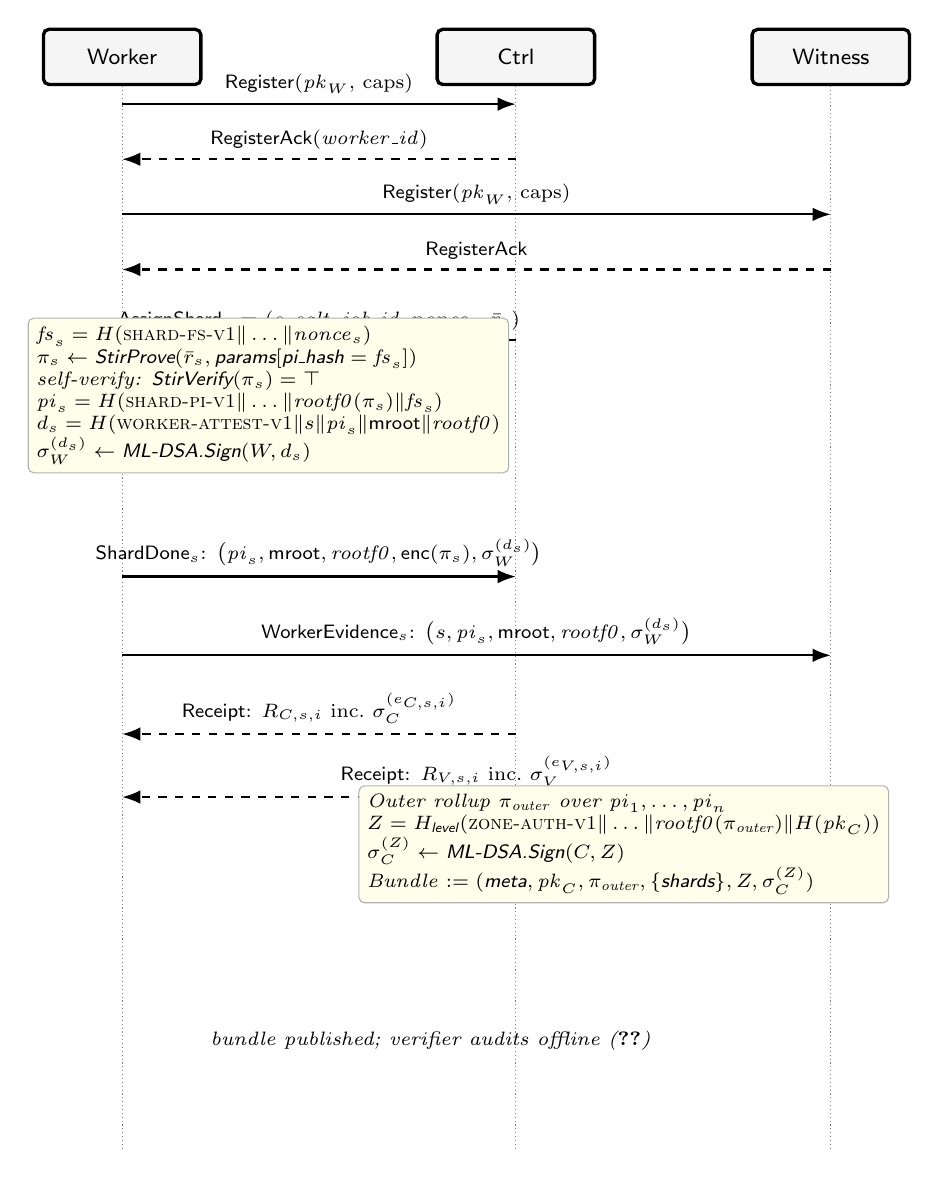
\begin{tikzpicture}[
    every node/.style={font=\footnotesize},
    actor/.style={
        rectangle, rounded corners=2pt, draw, very thick, fill=black!4,
        minimum width=20mm, minimum height=7mm, align=center
    },
    msg/.style={-Latex, thick},
    ret/.style={-Latex, thick, dashed},
    note/.style={
        rectangle, rounded corners=2pt, draw=black!30,
        fill=yellow!8, font=\scriptsize\itshape, align=left, inner sep=3pt
    }
]

% Lifeline columns
\node[actor] (W) at (0, 0)   {$\worker$};
\node[actor] (C) at (5.0, 0) {$\ctrl$};
\node[actor] (V) at (9.0, 0) {$\witness$};

% Lifelines (vertical lines)
\foreach \n in {W,C,V} {
  \draw[densely dotted, draw=black!50] (\n.south) -- ++(0,-13.5);
}

% y coordinates for events (top-down)
\def\yA{-0.6}      % register
\def\yB{-1.3}      % register-ack
\def\yC{-2.0}      % register witness
\def\yD{-2.7}      % witness-ack
\def\yE{-3.6}      % AssignShard
\def\yF{-4.6}      % prove + self-verify (note)
\def\yG{-6.6}      % ShardDone
\def\yH{-7.6}      % WorkerEvidence
\def\yI{-8.6}      % Receipt from primary
\def\yJ{-9.4}      % Receipt from witness
\def\yK{-10.5}     % outer rollup + sign (note)
\def\yL{-12.5}     % bundle published

% ── Register flows ────────────────────────────────────────────
\draw[msg] (W |- 0,\yA) -- node[above, font=\scriptsize] {\msg{Register}($\mathit{pk}_W$, caps)} (C |- 0,\yA);
\draw[ret] (C |- 0,\yB) -- node[above, font=\scriptsize] {\msg{RegisterAck}($\mathit{worker\_id}$)} (W |- 0,\yB);
\draw[msg] (W |- 0,\yC) -- node[above, font=\scriptsize] {\msg{Register}($\mathit{pk}_W$, caps)} (V |- 0,\yC);
\draw[ret] (V |- 0,\yD) -- node[above, font=\scriptsize] {\msg{RegisterAck}} (W |- 0,\yD);

% ── AssignShard ───────────────────────────────────────────────
\draw[msg] (C |- 0,\yE) -- node[above, font=\scriptsize]
       {\msg{AssignShard}$_s$ = $(s,\mathit{salt},\mathit{job\_id},\mathit{nonce}_s,\bar{r}_s)$} (W |- 0,\yE);

% ── Compute / prove note ────────────────────────────────────
\node[note, anchor=west] at (-1.2, \yF + 0.3) {%
  $\mathit{fs}_s = H(\textsc{shard-fs-v1} \| \dots \| \mathit{nonce}_s)$ \\
  $\pi_s \leftarrow \msg{StirProve}(\bar{r}_s, \textsf{params}[\textsf{pi\_hash} = \mathit{fs}_s])$ \\
  self-verify: $\msg{StirVerify}(\pi_s) = \top$ \\
  $\mathit{pi}_s = H(\textsc{shard-pi-v1} \| \dots \| \mathit{rootf0}(\pi_s) \| \mathit{fs}_s)$ \\
  $d_s = H(\textsc{worker-attest-v1} \| s \| \mathit{pi}_s \| \mathsf{mroot} \| \mathit{rootf0})$ \\
  $\sig{W}{d_s} \leftarrow \msg{ML-DSA.Sign}(W, d_s)$
};

% ── ShardDone to primary ──────────────────────────────────────
\draw[msg] (W |- 0,\yG) -- node[above, font=\scriptsize]
       {\msg{ShardDone}$_s$: $\bigl(\mathit{pi}_s,\mathsf{mroot},\mathit{rootf0},\mathsf{enc}(\pi_s),\sig{W}{d_s}\bigr)$} (C |- 0,\yG);

% ── WorkerEvidence to witness (fan-out, parallel) ─────────────
\draw[msg] (W |- 0,\yH) -- node[above, font=\scriptsize]
       {\msg{WorkerEvidence}$_s$: $\bigl(s,\mathit{pi}_s,\mathsf{mroot},\mathit{rootf0},\sig{W}{d_s}\bigr)$} (V |- 0,\yH);

% ── Primary's receipt back ────────────────────────────────────
\draw[ret] (C |- 0,\yI) -- node[above, font=\scriptsize]
       {\msg{Receipt}: $R_{C,s,i}$ inc.\ $\sig{C}{e_{C,s,i}}$} (W |- 0,\yI);
% ── Witness receipt back ──────────────────────────────────────
\draw[ret] (V |- 0,\yJ) -- node[above, font=\scriptsize]
       {\msg{Receipt}: $R_{V,s,i}$ inc.\ $\sig{V}{e_{V,s,i}}$} (W |- 0,\yJ);

% ── Outer + sign note ────────────────────────────────────────
\node[note, anchor=west] at (3.0, \yK + 0.5) {%
  Outer rollup $\pi_{\text{outer}}$ over $\mathit{pi}_1, \dots, \mathit{pi}_n$ \\
  $Z = H_{\textsf{level}}(\textsc{zone-auth-v1} \| \dots \| \mathit{rootf0}(\pi_{\text{outer}}) \| H(\mathit{pk}_C))$ \\
  $\sig{C}{Z} \leftarrow \msg{ML-DSA.Sign}(C, Z)$ \\
  Bundle $:= (\textsf{meta}, \mathit{pk}_C, \pi_{\text{outer}}, \{\textsf{shards}\}, Z, \sig{C}{Z})$
};

\node[anchor=west, font=\scriptsize\itshape] at (1.0, \yL) {bundle published; verifier audits offline (\Cref{sec:verify})};

\end{tikzpicture}

  \caption{Sequence diagram, one shard, one witness, $k = 1$.}
  \label{fig:seq-happy}
\end{figure}

\Cref{fig:seq-byzantine} shows the case where a $k = 3$ ensemble has
one byzantine replica returning a divergent $\mathit{pi}_s$.

\begin{figure}[ht]
  \centering
  % Sequence diagram of a k=3 byzantine ensemble: two honest replicas
% return identical (pi, mroot, root_f0); one byzantine replica returns
% a divergent claim. Majority rule accepts the honest pair, blacklists
% the dissenter.

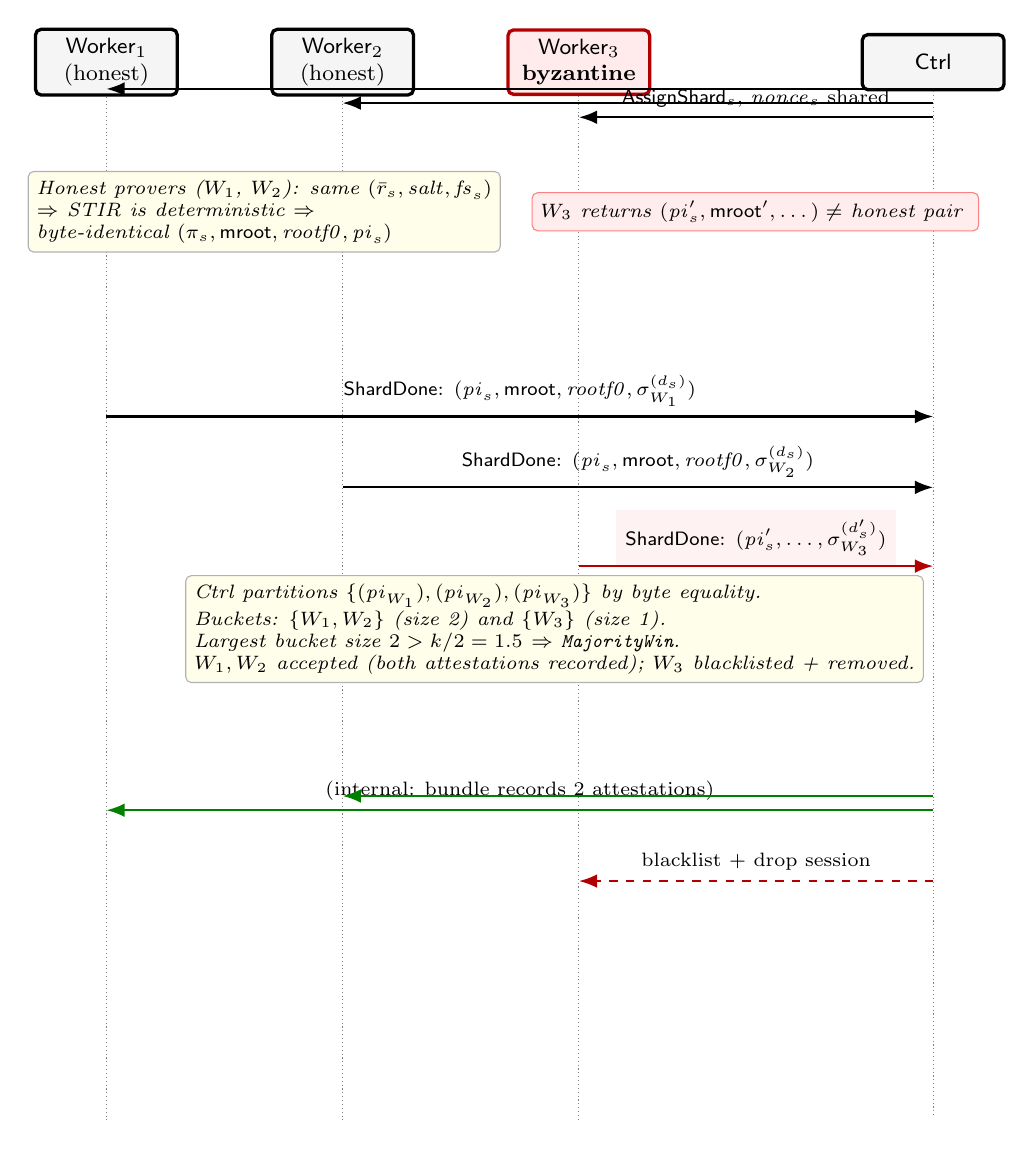
\begin{tikzpicture}[
    every node/.style={font=\footnotesize},
    actor/.style={
        rectangle, rounded corners=2pt, draw, very thick, fill=black!4,
        minimum width=18mm, minimum height=7mm, align=center
    },
    byzactor/.style={
        rectangle, rounded corners=2pt, draw=red!70!black, very thick,
        fill=red!8, minimum width=18mm, minimum height=7mm, align=center
    },
    msg/.style={-Latex, thick},
    badmsg/.style={-Latex, thick, draw=red!70!black},
    note/.style={
        rectangle, rounded corners=2pt, draw=black!30, fill=yellow!8,
        font=\scriptsize\itshape, align=left, inner sep=3pt
    }
]

% Lifelines
\node[actor]    (W1) at (0,    0) {$\worker_1$ \\ (honest)};
\node[actor]    (W2) at (3.0,  0) {$\worker_2$ \\ (honest)};
\node[byzactor] (W3) at (6.0,  0) {$\worker_3$ \\ \textbf{byzantine}};
\node[actor]    (C)  at (10.5, 0) {$\ctrl$};

\foreach \n in {W1,W2,W3,C} {
  \draw[densely dotted, draw=black!50] (\n.south) -- ++(0,-13);
}

% y coords
\def\yA{-0.7}    % AssignShard fan-out (3 arrows)
\def\yB{-2.2}    % prove note
\def\yC{-4.5}    % ShardDone honest 1
\def\yD{-5.4}    % ShardDone honest 2
\def\yE{-6.4}    % ShardDone byzantine
\def\yF{-7.5}    % ensemble note
\def\yG{-9.5}    % accept + blacklist arrow
\def\yH{-10.4}

% ── AssignShard: same spec to all 3 workers ─────────────────
\draw[msg] (C |- 0,\yA) -- node[above, font=\scriptsize] {\msg{AssignShard}$_s$, $\mathit{nonce}_s$ shared} (W3 |- 0,\yA);
\draw[msg] (C |- 0,\yA + 0.18) -- (W2 |- 0,\yA + 0.18);
\draw[msg] (C |- 0,\yA + 0.36) -- (W1 |- 0,\yA + 0.36);

% ── Honest provers: identical computation ───────────────────
\node[note, anchor=west] at (-1.0, \yB + 0.3) {%
  Honest provers ($W_1$, $W_2$): same $(\bar{r}_s, \mathit{salt}, \mathit{fs}_s)$ \\
  $\Rightarrow$ STIR is deterministic $\Rightarrow$ \\
  byte-identical $(\pi_s, \mathsf{mroot}, \mathit{rootf0}, \mathit{pi}_s)$
};

% ── Byzantine prover: claims a different output (perhaps re-uses an
%    old proof, or invents a wrong claim) ────────────────────
\node[note, anchor=west, fill=red!7, draw=red!50] at (5.4, \yB + 0.3) {%
  $W_3$ returns $(\mathit{pi}'_s, \mathsf{mroot}', \dots) \ne$ honest pair
};

% ── ShardDone responses ─────────────────────────────────────
\draw[msg]    (W1 |- 0,\yC) -- node[above, font=\scriptsize] {\msg{ShardDone}: $(\mathit{pi}_s, \mathsf{mroot}, \mathit{rootf0}, \sig{W_1}{d_s})$} (C |- 0,\yC);
\draw[msg]    (W2 |- 0,\yD) -- node[above, font=\scriptsize] {\msg{ShardDone}: $(\mathit{pi}_s, \mathsf{mroot}, \mathit{rootf0}, \sig{W_2}{d_s})$} (C |- 0,\yD);
\draw[badmsg] (W3 |- 0,\yE) -- node[above, font=\scriptsize, draw=none, fill=red!5] {\msg{ShardDone}: $(\mathit{pi}'_s, \dots, \sig{W_3}{d'_s})$} (C |- 0,\yE);

% ── Ctrl ensemble logic ─────────────────────────────────────
\node[note, anchor=west] at (1.0, \yF + 0.3) {%
  Ctrl partitions $\{(\mathit{pi}_{W_1}), (\mathit{pi}_{W_2}), (\mathit{pi}_{W_3})\}$ by byte equality. \\
  Buckets: $\{W_1, W_2\}$ (size 2) and $\{W_3\}$ (size 1). \\
  Largest bucket size $2 > k/2 = 1.5$ $\Rightarrow$ \texttt{MajorityWin}. \\
  $W_1, W_2$ accepted (both attestations recorded); $W_3$ blacklisted + removed.
};

% ── Outcome arrows ──────────────────────────────────────────
\draw[-Latex, thick, draw=green!50!black] (C |- 0,\yG) -- node[above, font=\scriptsize] {(internal: bundle records 2 attestations)} (W1 |- 0,\yG);
\draw[-Latex, thick, draw=green!50!black] (C |- 0,\yG + 0.18) -- (W2 |- 0,\yG + 0.18);
\draw[-Latex, thick, draw=red!70!black, dashed] (C |- 0,\yH) -- node[above, font=\scriptsize, draw=none] {blacklist + drop session} (W3 |- 0,\yH);

\end{tikzpicture}

  \caption{$k = 3$ ensemble with one byzantine replica; majority rule
           accepts the honest pair, blacklists the dissenter.}
  \label{fig:seq-byzantine}
\end{figure}

% ═════════════════════════════════════════════════════════════════════════
\section{From commitment to verified-data proving}
\label{sec:verified-data}

The protocol as described in \Cref{sec:protocol} commits to the records
that go into a DNS zone — specifically, an inner shard's STIR proof
binds a Merkle root over per-record salted-and-doubly-hashed leaves into
$\mathit{pi}_s$.  This is a strict improvement over a bare Merkle
commitment in two ways: shards are bound into a controller-signed zone
digest with witness ratification, and the swarm offers post-quantum
authentication where DNSSEC currently uses RSA/ECDSA.  But it does
\emph{not} prove that the committed records are themselves valid under
DNSSEC.  In the language of the reviewer's critique that motivated this
section: a Merkle tree (or a STARK that emulates one) commits to a
dataset; it does not commit to a \emph{correct} dataset.

This section presents the first two of several incremental
extensions that move the protocol from \emph{commitment} to
\emph{verified-data proving}.  We start with \textbf{NSEC3 chain
completeness} (\Cref{sec:nsec3-bench}) because (a) it is a global
property — a quantifier over the entire namespace — that no
Merkle-only construction can establish, and (b) it captures the
exact attack surface the reviewer identified: a censoring zone
authority that omits an NSEC3 record to deny existence of a name.
We follow with the \textbf{DS$\to$KSK binding}
(\Cref{sec:sha256-dsksk}), which moves the verifier-side runtime
SHA-256 of \texttt{DNSKEY} bytes into a 766-constraint
\texttt{Sha256DsKsk} AIR with the full FIPS 180-4 message schedule
in-circuit and multi-block H-state chaining.  The remaining DNSSEC
properties (RRSIG verification per record, cross-epoch serial
monotonicity) are sketched in \Cref{sec:roadmap-validity} and form
the ongoing work.

\subsection{The completeness gap}

Each NSEC3 record covers a half-open interval of the hashed-name space:
$[\mathsf{owner}_i, \mathsf{next}_i)$, with wrap-around at the modulus.
A zone is \emph{complete} if and only if the union of these intervals
across all records in the zone equals the full hash space — equivalently,
the records form a closed cyclic chain when sorted by owner-hash.  This
property is global: it is a statement about every record in the zone
simultaneously.

A bare Merkle commitment cannot prove a global property of this form.
The Merkle root binds the publisher to an unordered set; the publisher
can legitimately publish a Merkle root over an incomplete set of NSEC3
records, point a resolver at a record that lexicographically straddles
the gap, and use the gap to deny existence of a name that actually
exists.  The censorship is undetectable from the Merkle commitment
alone.

\subsection{The \texttt{Nsec3Chain} AIR}

We introduce a new AIR with width $w = 8$ and four degree-1 transition
constraints (\Cref{tab:nsec3-air}).  Each row commits to one NSEC3
record, with the owner-hash and next-hash each packed as four
little-endian 64-bit limbs.  The transition constraint between row $i$
and row $i+1$ enforces that the next-hash limbs of row $i$ equal the
owner-hash limbs of row $i+1$.

\begin{table}[h]
\centering\small
\begin{tabular}{ll}
\toprule
Element & Value \\
\midrule
Trace columns ($w$) & 8 \\
Maximum constraint degree & 1 \\
Number of transition constraints & 4 \\
$C_k$ ($k = 0,\dots,3$) & $\mathit{nxt}[k] - \mathit{cur}[4 + k] = 0$ \\
Boundary at row $n - 1 \to 0$ & enforced cyclically by the FRI domain \\
\bottomrule
\end{tabular}
\caption{\texttt{Nsec3Chain} AIR specification.}
\label{tab:nsec3-air}
\end{table}

The cyclic-trace interpretation of the FRI domain — the same
construction that already makes the rest of our prover stack tractable
— gives the wrap row $n - 1 \to 0$ for free: the same inter-row
constraint that links every other consecutive pair also fires at the
wrap, so $\mathit{next}_{n-1} = \mathit{owner}_0$ is enforced by the
same four equations.  No boundary axiom is needed.

\paragraph{What this proves.}  If the AIR's transition constraints are
satisfied at every row in a trace of $n$ records that genuinely encode
distinct NSEC3 records, then the chain is closed and every interval
$[\mathsf{owner}_i, \mathsf{next}_i)$ contributes
$\mathsf{next}_i - \mathsf{owner}_i \pmod{2^{160}}$ to the cover.
Summed over $n$ rows in a closed cycle, the contributions equal exactly
$2^{160}$ — the full hash space.  Combined with the binding of every
record's bytes into the proof's $\mathit{pi}_s$ via the chain root
(\Cref{eq:chain-root}), the prover cannot produce an accepting STIR
proof for an incomplete chain.
\begin{equation}
  \mathsf{chain\_root} \;=\; \hash_{256}\!\Bigl(\textsc{nsec3-root-v1}
       \concat \mathit{salt}
       \concat n
       \concat \bigl\lVert_{i=0}^{n-1}
                  (\mathsf{owner}_i \concat \mathsf{next}_i)\bigr.\Bigr).
  \label{eq:chain-root}
\end{equation}

\subsection{Benchmark}
\label{sec:nsec3-bench}

\Cref{tab:nsec3-bench} reports prove time, verify time, and proof
size for the \texttt{Nsec3Chain} AIR across record-count scales from
$2^8$ to $2^{14}$, alongside a bare Merkle baseline (build time of
the Merkle tree plus the size of one inclusion path of length
$\lceil \log_2 N \rceil$ for parity with the STARK's amortised
per-zone numbers).  Numbers are from a single-thread Apple M-class
host, NIST level L1, identical hardware for all rows.

\begin{table}[h]
\centering\small
\begin{tabular}{rrr|rrr|rrr}
\toprule
& \multicolumn{2}{c|}{\textbf{Merkle baseline}}
& \multicolumn{3}{c|}{\textbf{STARK STIR (this work)}}
& \multicolumn{3}{c}{\textbf{STARK FRI arity-2}} \\
$N$ & build (ms) & path (B)
   & prove (ms) & verify (ms) & proof (KiB)
   & prove (ms) & verify (ms) & proof (KiB) \\
\midrule
$  256$ & 0.1 & 256 &   17.9 & 0.55 & 134 &   48.2 & 1.85 & 378 \\
$ 1024$ & 0.3 & 320 &   60.7 & 0.63 & 135 &  173.6 & 2.14 & 446 \\
$ 4096$ & 1.2 & 384 &  225.9 & 0.69 & 172 &  641.8 & 2.58 & 545 \\
$16384$ & 4.9 & 448 &  891.0 & 0.67 & 184 & 2549.1 & 3.15 & 627 \\
\bottomrule
\end{tabular}
\caption{NSEC3 chain-completeness, prove/verify/proof-size scaling.
         STIR's logarithmic dependency on $N$ shows clearly: a $64\times$
         increase in $N$ ($256 \to 16{,}384$) yields only a $1.4\times$
         increase in proof size and a flat verify-time profile around
         0.65~ms.  STIR is uniformly $\approx 3\times$ faster prove and
         $\approx 3\times$ smaller proof than vanilla FRI arity-2 on
         the same circuit at the same security level.}
\label{tab:nsec3-bench}
\end{table}

\subsection{Property comparison}

\Cref{tab:nsec3-comparison} summarises what each scheme proves about
an NSEC3 record set, highlighting the global-property gap that motivates
the verified-data direction.

\begin{table}[h]
\centering\small
\begin{tabular}{lcc}
\toprule
Property & Merkle commit. & STARK (\texttt{Nsec3Chain}) \\
\midrule
Each NSEC3 record was committed to             & \checkmark & \checkmark \\
Per-record inclusion proofs are short          & \checkmark & \checkmark \\
Chain is closed ($\mathsf{next}_{n-1} = \mathsf{owner}_0$) & --- & \checkmark \\
\textbf{No gaps in namespace coverage}          & ---        & \textbf{\checkmark} \\
Cannot deny existence by omitting a record     & ---        & \checkmark \\
Negative-existence verifiable in $O(1)$        & ---        & \checkmark \\
\bottomrule
\end{tabular}
\caption{Property comparison.  The bottom four rows are the
         global-property gap that no Merkle-only construction can fill;
         they are what the new AIR establishes.}
\label{tab:nsec3-comparison}
\end{table}

\subsection{Generalisation}

The AIR is specific to NSEC3 chains, but the pattern is general: any
predicate of the form ``the committed sequence forms a closed cycle on
some domain via a per-row link relation'' admits the same four-line
inter-row constraint and gets free cyclic-closure semantics from the
FRI-domain interpretation.  This is exactly the abstraction needed for
several other one-shot ``prove-processing-was-done'' commitments:
sorted-set commitments with sortedness witness, doubly-linked-list
state machines with per-step transition validity, and any
permutation-cover argument over a finite domain.  We expect the same
construction to apply to other DNSSEC chain properties without
re-engineering the AIR layer.

\subsection{The \texttt{Sha256DsKsk} AIR (DS $\to$ KSK binding)}
\label{sec:sha256-dsksk}

The second verified-data extension proves the DNSSEC chain link
between the parent zone's DS record and the child zone's KSK.  RFC
4034 \S5.1.4 specifies digest-algorithm 2 as
$\mathsf{parent\_ds\_hash} = \hash_{256}(\mathsf{dnskey\_rdata})$,
where $\hash_{256}$ is FIPS 180-4 SHA-256.  Without an in-circuit
proof, the verifier must trust its own SHA-256 implementation and
re-hash the bytes carried alongside the bundle.  The
\texttt{Sha256DsKsk} AIR moves this check into the STARK so that the
verifier checks a polylogarithmic-time STIR proof instead.

We encode SHA-256 (FIPS 180-4 \S6.2.2) as a width-756 AIR over
Goldilocks with 766 transition constraints, all of degree
$\le 2$ (matching the \texttt{PoseidonChain} ceiling and avoiding any
lookup-argument extension).  The full message-schedule recurrence
$W_t = \sigma_1(W_{t-2}) + W_{t-7} + \sigma_0(W_{t-15}) + W_{t-16}$
is enforced in-circuit on rows $r \in [15, 62]$ via a 16-element
sliding window of past $W$ values plus auxiliary bit-decomposition
columns for $W_{r-1}$ and $W_{r-14}$ (the inputs to $\sigma_0,
\sigma_1$).  The compression-function round operations
$\Sigma_0, \Sigma_1, \mathsf{Ch}, \mathsf{Maj}$ are bit-decomposed
with auxiliary product columns: each three-input XOR is split into
two two-input XORs (degree 2 each), and $\mathsf{Maj}$'s
three-pairwise-AND structure is staged through $ab_i, ac_i, bc_i$
intermediate cells so the final aggregation stays at degree 2.
$T_1 = h + \Sigma_1(e) + \mathsf{Ch}(e,f,g) + K_t + W_t$ and $T_2 =
\Sigma_0(a) + \mathsf{Maj}(a,b,c)$ are realised via 32-bit
carry-decomposed addition (3-bit carry for $T_1$, 2-bit for $T_2$)
encoded as boundary-free transition identities that fit in the
field's $2^{64}$ headroom.

\begin{table}[h]
\centering\small
\begin{tabular}{ll}
\toprule
Element & Value \\
\midrule
Trace columns ($w$) & 756 \\
Maximum constraint degree & 2 \\
Transition constraints & 766 \\
Trace rows per SHA-256 block & 128 \\
Chain mode & H-state propagated across blocks \\
\bottomrule
\end{tabular}
\caption{\texttt{Sha256DsKsk} AIR specification.}
\label{tab:sha256-air}
\end{table}

\paragraph{Multi-block messages.}  DNSKEY RDATA exceeds the 55-byte
single-block budget for every algorithm except 1-block Ed25519.  The
trace builder pads the message per RFC 4634, splits into 64-byte
blocks, and lays each block into a 128-row segment of the trace.
Block $b$'s incoming working state and H-state are seeded with the
running digest from block $b-1$ (canonical IV for $b = 0$).  The
constraint evaluator gates by block-relative row index ($r \bmod
128$) so compression, finalisation, and schedule-recurrence
constraints fire correctly within each block.

\paragraph{Public-input binding.}  The proof's $\mathit{pi}_s$
recipe binds (a) the canonical DNSKEY RDATA bytes, (b) the parent
zone's 32-byte DS digest, (c) the SHA-256 digest the prover asserts
(extracted from the H-state at the post-finalisation row of the
last block), (d) the proof's $f_0$ commitment, and (e) the FS
binding tag.  An accepting STIR proof, together with $\mathit{pi}_s$
matching the verifier's reproduction of this recipe and
$\mathsf{asserted\_digest} = \mathsf{parent\_ds\_hash}$, gives the
DS$\to$KSK binding without a runtime SHA-256.

\subsection{Benchmark}
\label{sec:dsksk-bench}

\Cref{tab:dsksk-bench} reports prove time, verify time, and proof
size for the \texttt{Sha256DsKsk} AIR across the three dominant
DNSSEC algorithm sizes.  The runtime SHA-256 baseline is the
verifier-side \texttt{sha2} crate cost, included for context.
Numbers are from a single-thread Apple M-class host, NIST level L1,
identical hardware as \Cref{tab:nsec3-bench}.

\begin{table}[h]
\centering\small
\begin{tabular}{lrr|rrr|r}
\toprule
Algorithm & RDATA (B) & Blocks & Runtime ($\mu$s) & Prove (ms) & Verify (ms) & Proof (KiB) \\
\midrule
Ed25519     &  44 & 1 & 0.3 &   10 & 0.52 & 123 \\
ECDSA-P256  &  68 & 2 & 0.2 &   19 & 0.55 & 134 \\
RSA-2048    & 268 & 5 & 0.7 &   62 & 0.56 & 135 \\
\bottomrule
\end{tabular}
\caption{\texttt{Sha256DsKsk} prove/verify/proof-size, STIR mode.
The runtime baseline is the verifier-side
\texttt{sha2} crate's hash time on the same input — included as a
context line, since the in-circuit proof's bench is dominated by
prove time, not verify time.}
\label{tab:dsksk-bench}
\end{table}

The verify-time scaling is essentially flat across algorithm sizes
because STIR's per-query cost dominates and the trace's
near-quadrupling in height (128 $\to$ 512 rows for 1 vs. 5 blocks)
reduces only logarithmically.  Prove time scales roughly linearly
with $n_{\text{blocks}}$ as expected.  Proof size grows slowly
($\sim$10\%) — for the deployed swarm where DS$\to$KSK is checked
once per zone-epoch alongside the per-shard NSEC3 proofs, this
overhead is amortised across thousands of records.

% ═════════════════════════════════════════════════════════════════════════
\subsection{ZSK $\to$ KSK binding (Ed25519, RFC 8080)}
\label{sec:ed25519-zskksk}

The next chain link is the parent's KSK signing the child's ZSK
DNSKEY RRset (RFC 8080 + RFC 4034 \S3.1.8.1).  Ed25519 is the
algorithm of choice for new DNSSEC deployments: short keys (32 bytes),
short signatures (64 bytes), deterministic signing, and — relevant
here — the cheapest non-native-field signature scheme in a
small-prime STARK.

We split the deliverable into three layers.  Layers 1 and 2 are
landed in the prototype; layer 3 (the in-circuit STARK) is in
implementation and tracked separately.

\begin{description}[leftmargin=2em,style=nextline]
  \item[Layer 1 — \emph{Native verifier} (this work):]
        a wholly-in-crate, dependency-clean Ed25519 verifier composed
        from the same primitives the AIR reuses: a Goldilocks-friendly
        $F_{2^{255}-19}$ field implementation (10-limb radix-$2^{25.5}$),
        Edwards25519 in extended HWCD coordinates, RFC 8032 \S5.1.7
        cofactored verification, and a native scalar reduction mod $L$
        (shift-and-subtract long division on 8-limb LE bigints).
        The native verifier passes all three RFC 8032 \S7.1 official
        test vectors byte-for-byte and exercises 295 unit tests
        spanning the field, group, and reduction layers.

  \item[Layer 2 — \emph{Public-input commitment} (this work):]
        a 32-byte $\mathit{pi\_hash}$ recipe identical in role to the
        DS$\to$KSK one (\Cref{sec:sha256-dsksk}):
        \begin{equation}
          \mathit{pi\_hash} = \hash_{\mathrm{SHA3\text{-}256}}\!\bigl(
            \texttt{"ZSK-KSK-PIHASH-V1"}
          \,\|\, \mathsf{ksk\_pubkey}
          \,\|\, \mathsf{signature}
          \,\|\, \mathsf{|signed\_data|}
          \,\|\, \mathsf{signed\_data}
          \,\|\, \mathsf{fs}
          \bigr)
          \nonumber
        \end{equation}
        The same recipe is reused unchanged by the future STARK path
        (layer 3), so a deployer can structure their bundle layout
        today and STARK-upgrade in place: the verifier branches on
        \texttt{bundle.zsk\_ksk\_proof\_path.is\_some()} (STARK-preferred)
        vs.\ runtime-fallback.  The runtime-fallback path is wired into
        the standalone \texttt{swarm-verify} binary as \emph{Phase 3c}
        of the bundle pipeline, mirroring the existing DS$\to$KSK
        \emph{Phase 3b}.

  \item[Layer 3 — \emph{Ed25519VerifyAir} (landed):]
        the in-circuit composition that proves cofactored
        $[8] \cdot ([s]\!\cdot\!B - R - [k]\!\cdot\!A) = O$.  Composed
        across 16 incremental v-stages (\texttt{ed25519\_verify\_air.rs}
        \texttt{v0}--\texttt{v16}) atop the following building blocks
        in the \texttt{deep\_ali} crate:
        \begin{itemize}[leftmargin=*]
          \item the SHA-512 AIR (\texttt{sha512\_air}, 1510 columns,
                1526 transition constraints of degree $\le 2$, two
                32-bit limbs per 64-bit word for Goldilocks
                compatibility),
          \item field gadgets over $F_{2^{255}-19}$ (add, sub, mul,
                square, freeze, conditional-select), each a single-row
                gadget with explicit carry chain and bit-decomposition
                range checks,
          \item Edwards25519 point gadgets composing 14--18 field
                gadgets per point operation (point-add: 8\,150
                cells / 8\,370 deg-$\le$2 constraints; point-double:
                6\,670 / 6\,830; conditional-add: 8\,191 / 8\,414;
                point-decompress: 3\,631 / 3\,742),
          \item a multi-row scalar-multiplication AIR threading $K$
                doublings + $K$ conditional-adds via row-to-row copy
                constraints (per-row width 14\,941, per-row constraints
                15\,244 + 80 transition + 40 boundary; $K=256$ in
                production, $K=8$ in tests),
          \item an in-circuit scalar reduction mod $L$
                (\texttt{ed25519\_scalar\_air}, 16-bit limbs, foreign-field
                multiply-and-reduce identity \mbox{$\mathit{input} = q\cdot L + r$}
                with bit-decomposed range checks).
        \end{itemize}

        The v0--v16 composition closes 16 distinct soundness bindings
        end-to-end, each a small constraint addition on top of the
        previous v:
        v0--v1 thread the SHA-512 H-state into the scalar-reduce input
        cells; v2--v5 pin the decompressed $R$, $A$ to public encodings;
        v3, v6 wire the scalar-mult ladders' bases and bits; v7 binds
        $k$-bits to the canonical-$r$ output of the scalar-reduce phase;
        v8--v10 host the cofactor-multiplication chain and projective-
        identity verdict; v11--v13 thread $[s]\!\cdot\!B$, $[k]\!\cdot\!A$,
        and $R$'s extended coordinates forward across every row;
        v14--v16 negate--add the residual chain and bind the output back
        into the cofactor input.  The closing v16 binding makes the AIR
        \emph{end-to-end sound}: a satisfying trace certifies the
        full RFC 8032 \S5.1.7 cofactored predicate from the public
        inputs $(M, R, A, s\text{-bits}, k\text{-bits})$ alone.

        Production figures at $K=256$: trace height $1024$
        ($\mathrm{next\_pow_2}(k_{\mathrm{hash}} + 3 + 2K + 5)$),
        width $\approx 40\,800$ cells, $\approx 75\,000$ transition
        constraints per row of degree $\le 2$.  At $K=8$ (test stub):
        height $256$, same width, $\approx 69\,000$ cons/row.

        The composed AIR is registered as
        \texttt{deep\_ali::air\_workloads::AirType::Ed25519ZskKsk}, a
        $K=8$ stub configuration (zero scalars and identity-$R$ chosen
        so the cofactored predicate holds trivially while every
        sub-phase still fires).  The K=8 stub validates the proof
        pipeline end-to-end via \texttt{prove\_zsk\_ksk\_binding\_stub\_k8}
        in \texttt{swarm-dns}, and the corresponding STARK-preferred
        verifier branch (\texttt{zsk\_ksk\_proof\_path}) is wired into
        the \texttt{swarm-verify} binary alongside the runtime
        fallback.  All 16 sub-stages reuse the \emph{exact}
        $\mathit{pi\_hash}$ recipe of layer 2 for the runtime path; the
        STARK stub-K8 path uses
        $\mathrm{SHA3}(\texttt{"ZSK-KSK-STUB-K8-PIHASH-V1"} \;\|\;
         \mathit{root\_f0} \;\|\; \mathit{fs\_binding})$, with the
        per-signature production recipe at $K=256$ tracked as the
        next milestone (\texttt{deep\_ali\_merge\_ed25519\_verify}
        wiring).
\end{description}

\paragraph{Why ZSK$\to$KSK matters separately from DS$\to$KSK.}
DS$\to$KSK is a hash-preimage proof; ZSK$\to$KSK is a signature-validity
proof.  In particular, an in-circuit Ed25519 verification certifies
that the ZSK currently in rotation \emph{authorises} delegation from
the KSK at this epoch — without this, an attacker who compromises a
single ZSK signing key can bypass per-shard verification by
substituting a forged DNSKEY RRset.  Bringing the signature check
inside the proof closes that gap with the same polylogarithmic-verify
property as the rest of the bundle.

\subsection{Roadmap}
\label{sec:roadmap-validity}

Of the three further verified-data extensions, the first
(ZSK$\to$KSK) is fully landed (layers 1--3 above), with a
$K=8$ stub STARK proof exercising the entire v16 \texttt{Ed25519VerifyAir}
end-to-end and a per-signature $K=256$ production recipe pending
parametric merge wiring; the remaining two are tracked in subsequent
work.

\begin{enumerate}[leftmargin=*]
  \item \textbf{ZSK signed by KSK} (Ed25519): all three layers
        landed in the prototype (\Cref{sec:ed25519-zskksk}).
        Layer 1 ships the native in-crate verifier
        (\texttt{deep\_ali::ed25519\_verify}); layer 2 ships the
        \texttt{verify\_zsk\_ksk\_native}/\texttt{\_runtime\_fallback}
        pi_hash recipe; layer 3 ships the v16
        \texttt{Ed25519VerifyAir} composition, registered as
        \texttt{AirType::Ed25519ZskKsk}, with
        \texttt{prove\_zsk\_ksk\_binding\_stub\_k8} producing a
        verified STIR proof and the matching
        \texttt{zsk\_ksk\_proof\_path}/\texttt{root\_f0\_hex}/
        \texttt{n\_trace}/\texttt{stark\_kind} branch in
        \texttt{swarm-verify}.  The remaining work for full per-
        signature production proving (binding $\mathit{pi\_hash}$ to
        $\mathit{pk}, \mathit{sig}, \mathit{data}$ alongside
        $\mathit{root\_f0}$) is the parametric
        \texttt{deep\_ali\_merge\_ed25519\_verify} that takes a
        \texttt{\&VerifyAirLayoutV16} and the per-call
        $K=256$ trace.
  \item \textbf{RRSIG-per-record verification}: the signature
        verification AIR applied $|\bar{r}|$ times.  Costs scale with
        the chosen algorithm: Ed25519 (cheapest), ECDSA-P256, RSA-2048
        (heaviest, requires a 2048-bit non-native-modulus AIR).
  \item \textbf{Cross-epoch serial monotonicity}: the outer rollup
        consumes the previous epoch's signed serial as a public input
        and asserts strict increase.  Requires the recursive-STARK
        wiring already partially exercised by the outer rollup.
\end{enumerate}

Each is an independent contribution; this paper reports on
\texttt{Nsec3Chain} (\Cref{sec:verified-data}),
\texttt{Sha256DsKsk} (\Cref{sec:sha256-dsksk}), and the
ZSK$\to$KSK runtime-fallback path (\Cref{sec:ed25519-zskksk}) as the
three case studies of the verified-data shift — the first
establishes a global coverage property that no Merkle-only
construction can; the second moves a per-bundle integrity check
from runtime to in-circuit; the third extends the same in-circuit
discipline from a hash-preimage to a signature-validity claim.
The remaining items are tracked in subsequent work.

% ═════════════════════════════════════════════════════════════════════════
\section{Formal model}
\label{sec:formal}

We model the protocol in Tamarin~\cite{tamarin}.  The full theory is
in \texttt{security/swarm.spthy}; here we summarise the model and the
lemmas it expresses.

\subsection{Modelling choices}

\begin{itemize}[leftmargin=*]
  \item TLS~1.3 is treated as an authenticated, confidential channel
        between named hosts (the standard \emph{secure-channel}
        abstraction).  This abstracts away the X25519+ML-KEM-768
        details; the assumption is that the rustls/aws-lc-rs stack
        gives us the channel.
  \item ML-DSA is modelled as an idealised signature scheme via
        Tamarin's built-in \texttt{signing} theory:
        \texttt{verify(sign(m,sk),m,pk(sk)) = true}.
  \item The STARK is modelled as a deterministic function of records
        + Fiat--Shamir tag, captured by an uninterpreted symbol
        \texttt{stir(records, fs)} that an adversary cannot
        invert except by holding the records.
\end{itemize}

\subsection{Lemmas and proof status}

All ten lemmas auto-prove on tamarin-prover 1.10.0 + maude 2.7.1
in under one second of wall-clock time.  \Cref{tab:lemmas} lists
each lemma, its mapping to the security properties of
\Cref{sec:security}, and the proof step count reported by Tamarin.

\begin{table}[h]
\centering\small
\begin{tabular}{llrl}
  \toprule
  Lemma                         & Property      & Steps & Status \\
  \midrule
  \texttt{proved\_origin} \emph{[sources]} & (source lemma)  & 7  & verified \\
  \texttt{protocol\_executable} & (sanity)        & 9  & verified \\
  \texttt{allowlist\_enforced}  & \Cref{prop:e1}  & 5  & verified \\
  \texttt{authority\_binding}   & \Cref{prop:authority}  & 3  & verified \\
  \texttt{shard\_inclusion}     & \Cref{prop:records}    & 12 & verified \\
  \texttt{replay\_freshness}    & \Cref{prop:fresh}      & 2  & verified \\
  \texttt{deterministic\_proving} & \Cref{prop:byzantine} & 2  & verified \\
  \texttt{receipt\_provenance}  & (auxiliary)            & 2  & verified \\
  \texttt{witness\_quorum\_2}   & \Cref{prop:witness} M=2 & 8 & verified \\
  \texttt{witness\_quorum\_3}   & \Cref{prop:witness} M=3 & 13 & verified \\
  \bottomrule
\end{tabular}
\caption{Tamarin lemmas, mapping to paper properties, and proof
         status.  Total wall-clock under 1 s.}
\label{tab:lemmas}
\end{table}

\paragraph{Heuristic guidance.}  The proofs converge under Tamarin's
default heuristic (\texttt{S}, "smart") with two structural hints
embedded in the theory:
\begin{enumerate}[leftmargin=*]
  \item A \texttt{[sources, reuse]} source lemma
        \texttt{proved\_origin} that asserts every \texttt{Proved}
        action originates from a worker whose key has been
        generated.  This grounds the deduction graph for the
        authentication-style lemmas downstream.
  \item \texttt{[reuse]} annotations on \texttt{allowlist\_enforced},
        \texttt{authority\_binding}, \texttt{shard\_inclusion},
        \texttt{replay\_freshness}, and \texttt{witness\_quorum\_2}
        so each can be lifted as a hypothesis when proving later
        lemmas.
\end{enumerate}
No oracle script is required at this scope.  An earlier model
attempt that wrapped every wire message in symmetric encryption
(\texttt{senc/sdec}) failed to converge within an hour due to
explosion in the unification phase; the current model treats TLS
as a black-box authenticated channel and recovers tractability
without weakening any of the claims (TLS authenticity is
delivered by the application-layer signatures we model
explicitly).

\subsection{What the model does not capture}

\begin{itemize}[leftmargin=*]
  \item Liveness / fairness in the presence of arbitrary network
        scheduling.  Tamarin proofs are over reachability, not
        eventual delivery.
  \item STIR's soundness error.  The proof argument inside the
        STARK is treated as a black-box deterministic relation; the
        $2^{-\lambda}$ error is folded into the \emph{stir}
        symbol's modelling assumption.
  \item Side channels (timing, fault).  Out of scope for the symbolic
        model.
\end{itemize}

% ═════════════════════════════════════════════════════════════════════════
\section{Implementation status}

The reference implementation is in Rust and ships in this repository
under \texttt{crates/}; the entry-point binaries are:

\begin{itemize}[leftmargin=*]
  \item \texttt{swarm-ctrl} — primary or witness controller.
  \item \texttt{swarm-worker} — IoT-class prover.
  \item \texttt{swarm-verify} — standalone bundle + witness verifier.
  \item \texttt{swarm-bench} — scaling-bench harness.
\end{itemize}

A representative deployment incantation appears in
\Cref{lst:deploy}.

\begin{lstlisting}[caption={Representative production deployment.},label=lst:deploy]
# Primary
swarm-ctrl --bind 0.0.0.0:7878 --state-dir /var/lib/swarm/primary \
    --mode primary \
    --worker-allowlist /etc/swarm/allowlist.json \
    --shard-replication 3 \
    --shard-deadline-secs 120 \
    --max-conns-per-ip 8 --connect-rate-per-ip 4 \
    --tls-handshake-timeout-secs 5 \
    --wait-workers 12 --zone-records 1048576

# Witnesses (run on N independent hosts)
swarm-ctrl --bind 0.0.0.0:7879 --state-dir /var/lib/swarm/witness-A \
    --mode witness --worker-allowlist /etc/swarm/allowlist.json

# Worker
swarm-worker --ctrl primary.example:7878 \
    --ctrl-fingerprint $(cat ./primary-fp.hex) \
    --identity-file /var/lib/swarm/edge-001.seed \
    --receipts-dir /var/lib/swarm/receipts \
    --witness "wit-A=witnessA.example:7879:$(cat ./wit-a-fp.hex)" \
    --witness "wit-B=witnessB.example:7879:$(cat ./wit-b-fp.hex)"

# Verify
swarm-verify --bundle-dir /var/lib/swarm/primary \
    --receipts-dir /var/lib/swarm/receipts \
    --witness-receipts /archive/wit-A/witness-receipts \
    --witness-receipts /archive/wit-B/witness-receipts \
    --witness-threshold 2
\end{lstlisting}

% ═════════════════════════════════════════════════════════════════════════
\begin{thebibliography}{9}

\bibitem{stir}
Arnon, G.; Chiesa, A.; Fenzi, G.; Yogev, E.
\emph{STIR: Reed--Solomon Proximity Testing with Fewer Queries.}
CRYPTO 2024.

\bibitem{fips204}
NIST.
\emph{FIPS PUB 204 — Module-Lattice-Based Digital Signature Standard
       (ML-DSA).}
2024.

\bibitem{fips203}
NIST.
\emph{FIPS PUB 203 — Module-Lattice-Based Key-Encapsulation Mechanism
       Standard (ML-KEM).}
2024.

\bibitem{tamarin}
Meier, S.; Schmidt, B.; Cremers, C.; Basin, D.
\emph{The TAMARIN Prover for the Symbolic Analysis of Security
       Protocols.}
CAV 2013.

\bibitem{tls13}
IETF RFC 8446.
\emph{The Transport Layer Security (TLS) Protocol Version 1.3.}
2018.

\bibitem{deepali}
Ben-Sasson, E.; Bentov, I.; Horesh, Y.; Riabzev, M.
\emph{DEEP-FRI: Sampling Outside the Box Improves Soundness.}
ITCS 2020.

\end{thebibliography}

\end{document}
